%%%%%%%%%%%%%%%%%%%%%%%%%%%%%%%%%%%%%%%%%%%%%%%%%%%%%%%%%%%%%%%%%%%%%%%%%%%%%%%%
%2345678901234567890123456789012345678901234567890123456789012345678901234567890
%        1         2         3         4         5         6         7         8
%% PP_Report.tex
%% V2.1
%% 2017/05/07
%% by Rui Santos Cruz
%% This is a skeleton file using PPIEEEtran.cls
%% (requires PPIEEEtran.cls) 
% !TEX root = ./main.tex
%%%%%%%%%%%%%%%%%%%%%%%%%%%%%%%%%%%%%%%%%%%%%%%%%%%%%%%%%%%%%%%%%%%%%%%%%%%%%%%%
\documentclass[a4paper,12pt,journal,twoside,compsoc]{PPIEEEtran}

% In the ReportType command chose "act" for Activity Report or "learn" for Learnings Report
\newcommand*{\ReportType}{act}
% -----------------------------------------------------------------------------
% The Preamble document contains all the necessary Packages for typesetting
% Modify it to suit your needs
% -----------------------------------------------------------------------------
%%%%%%%%%%%%%%%%%%%%%%%%%%%%%%%%%%%%%%%%%%%%%%%%%%%%%%%%%%%%%%%%%%%%%%%%%%%%%%%%
%2345678901234567890123456789012345678901234567890123456789012345678901234567890
%        1         2         3         4         5         6         7         8
% Required Packages and commands
% --> Please Choose the MAIN LANGUAGE for the document in package BABEL (below)
% --> Please Choose the TYPE OF REPORT for the document in \ReportType (below)
% !TEX root = ./main.tex
% PP_Report_Preamble.tex
% V2.1
% 2017/05/07
% by Rui Santos Cruz
%%%%%%%%%%%%%%%%%%%%%%%%%%%%%%%%%%%%%%%%%%%%%%%%%%%%%%%%%%%%%%%%%%%%%%%%%%%%%%%%
%
% *** INPUT LANGUAGE PACKAGES ***
% Choose the main language in package Babel
\usepackage[english,main=portuguese]{babel}
\usepackage[utf8]{inputenc}
\usepackage{iflang}

% *** ACRONYM PACKAGES ***
% Put definition of Acronyms at the end of the document
\usepackage[printonlyused,nolist]{acronym}

% *** CITATION PACKAGES ***
\usepackage{cite}

% *** GRAPHICS RELATED PACKAGES ***
\usepackage[pdftex]{graphicx}
\DeclareGraphicsExtensions{.pdf,.jpeg,.png}

% *** MATH PACKAGES ***
\usepackage[cmex10]{amsmath}

% *** SPECIALIZED LIST PACKAGES ***
\usepackage{algorithmic}

% *** ALIGNMENT PACKAGES ***
\usepackage{array}

% *** SUBFIGURE PACKAGES ***
\usepackage[caption=false,font=normalsize,labelfont=sf,textfont=sf]{subfig}

% *** FLOAT PACKAGES ***
\usepackage{fixltx2e}

% *** PDF, URL AND HYPERLINK PACKAGES ***
\usepackage{url}

% *** BACKGROUND Material ***
\usepackage{eso-pic}
\usepackage[
  contents={},
  opacity=1,
  scale=1,
  color=blue!90
  ]{background}
  
% *** CONDITIONALS ***
\usepackage{ifthen}

% Clever Referencing
% Note: portuguese is supported through "brazilian" option
\usepackage[\IfLanguageName{english}{english}{brazilian}]{cleveref}

%%%%%%%%%%%%%%%%%%%%%%%%%%%%%%%%%%%%%%%%%%%%%%%%%%%%%%%%%%%%%%%%%%%%%%%%%%%%%%%%
% PLEASE DO NOT CHANGE THIS SECTION
% Printing the Scoring Table
\AddToShipoutPicture*{\BackgroundPic}
%%%%%%%%%%%%%%%%%%%%%%%%%%%%%%%%%%%%%%%%%%%%%%%%%%%%%%%%%%%%%%%%%%%%%%%%%%%%%%%%
% PLEASE DO NOT CHANGE THIS SECTION
% Print Vertical Identifications on even and odd pages
\AddEverypageHook{%
  \ifthenelse{\isodd{\value{page}}}%
  {\backgroundsetup{
    angle=90,
    position={-0.1\textwidth,-1.055\textheight},
    contents={\tiny{PP-2017 V2.1}}
    }% Odd Pages
  }%
  {\backgroundsetup{
    angle=90,
    position={0.97\textwidth,-1.05\textheight},%
    contents={\ifthenelse{\equal{\ReportType}{act}}{%
              \tiny{\tlangRepActivity}}{\tiny{\tlangRepLearning}}}
    }% Even Pages
  }%
  \BgMaterial}
  %%%%%%%%%%%%%%%%%%%%%%%%%%%%%%%%%%%%%%%%%%%%%%%%%%%%%%%%%%%%%%%%%%%%%%%%%%%%%%%%
% correct bad hyphenation here
\hyphenation{op-tical net-works semi-conduc-tor}
%%%%%%%%%%%%%%%%%%%%%%%%%%%%%%%%%%%%%%%%%%%%%%%%%%%%%%%%%%%%%%%%%%%%%%%%%%%%%%%%
%2345678901234567890123456789012345678901234567890123456789012345678901234567890
%        1         2         3         4         5         6         7         8
\begin{document}

%%%%%%%%%%%%%%%%%%%%%%%%%%%%%%%%%%%%%%%%%%%%%%%%%%%%%%%%%%%%%%%%%%%%%%%%%%%%%%%%
%2345678901234567890123456789012345678901234567890123456789012345678901234567890
%        1         2         3         4         5         6         7         8
%% PP_Report_Cover.tex
%% V2.1
%% 2017/05/07
%% by Rui Santos Cruz
% !TEX root = ./main.tex
%%%%%%%%%%%%%%%%%%%%%%%%%%%%%%%%%%%%%%%%%%%%%%%%%%%%%%%%%%%%%%%%%%%%%%%%%%%%%%%%
% paper title
% can use linebreaks \\ within to get better formatting as desired
% Do not put math or special symbols in the title.
\title{Deteção de eventos em discursos políticos}

%%%%%%%%%%%%%%%%%%%%%%%%%%%%%%%%%%%%%%%%%%%%%%%%%%%%%%%%%%%%%%%%%%%%%%%%%%%%%%%%
% Author names
%
% note positions of commas and nonbreaking spaces ( ~ ) LaTeX will not break
% a structure at a ~ so this keeps an author's name from being broken across
% two lines.
% use \thanks{} to gain access to the first footnote area
% a separate \thanks must be used for each paragraph.
%
%\IEEEcompsocitemizethanks is a special \thanks that produces the bulleted
% lists for "first footnote" author affiliations. 
% Use \IEEEcompsocthanksitem which works much like \item
% for each affiliation group.
\author{Gonçalo~Fialho~Pires,
        Pedro~Miguel~Duarte% <-this % stops a space
% Change the Course Name 
% note: need leading \protect in front of \\ to get a newline within \thanks as
% \\ is fragile and will error, could use \hfil\break instead.
\IEEEcompsocitemizethanks{
\IEEEcompsocthanksitem Gonçalo~Fialho~Pires, nr. 79112,\protect\\ 
E-mail: goncalo.f.pires@tecnico.ulisboa.pt,
\IEEEcompsocthanksitem Pedro~Duarte, nr. 78328,\protect\\
E-mail: pedro.m.duarte@tecnico.ulisboa.pt,\protect\\
Instituto Superior Técnico, Universidade de Lisboa.\protect\\}% <-this % stops an unwanted space}% <-this % stops an unwanted space
\thanks{Manuscrito recebido a 1 de Junho de 2018.}
}
%%%%%%%%%%%%%%%%%%%%%%%%%%%%%%%%%%%%%%%%%%%%%%%%%%%%%%%%%%%%%%%%%%%%%%%%%%%%%%%%
% The paper headers
\markboth{Deteção de eventos em discursos políticos}%
% for a single student
%{Surname}% : for a single student 
% for a Group Report 
{Duarte \MakeLowercase{\textit{et al.}}}% : for a Group Report 
%
% The only time the second header will appear is for the odd numbered pages
% after the title page when using the twoside option.

%%%%%%%%%%%%%%%%%%%%%%%%%%%%%%%%%%%%%%%%%%%%%%%%%%%%%%%%%%%%%%%%%%%%%%%%%%%%%%%%
% Prints in Subtitle the type of Report
% PLEASE DO NOT CHANGE THIS SECTION
\IEEEspecialpapernotice{%
\ifthenelse{\equal{\ReportType}{act}}{%
\tlangRepActivity}{\tlangRepLearning}
}
%%%%%%%%%%%%%%%%%%%%%%%%%%%%%%%%%%%%%%%%%%%%%%%%%%%%%%%%%%%%%%%%%%%%%%%%%%%%%%%%
%%%%%%%%%%%%%%%%%%%%%%%%%%%%%%%%%%%%%%%%%%%%%%%%%%%%%%%%%%%%%%%%%%%%%%%%%%%%%%%%
% The paper Abstract and Keywords
\IEEEtitleabstractindextext{%

\begin{abstract}
Este relatório descreve as tarefas realizadas em colaboração com o Professor Nuno Mamede pertencente ao INESC-ID (Investigação e Desenvolvimento) e cujo seu foco assenta em desenvolver ferramentas para ajudar os utilizadores na análise de corpus de cariz político de forma a identificar alguns dos eventos mais frequentes. Para além deste trabalho foi também desenvolvida outra ferramenta que permite analisar frases e recolher o tipo de pronomes da mesma. Este tipo de atividades permitiu não só aos autores aprender novas tecnologias mas também possibilitou pôr em prática o sentido de responsabilidade num contexto profissional.

\end{abstract}
%
\begin{IEEEkeywords}
IST, INESC-ID, STRING, análise de corpus, pronomes, contexto profissional
\end{IEEEkeywords}}
%%%%%%%%%%%%%%%%%%%%%%%%%%%%%%%%%%%%%%%%%%%%%%%%%%%%%%%%%%%%%%%%%%%%%%%%%%%%%%%%

% make the title area
\maketitle

\IEEEdisplaynontitleabstractindextext
\IEEEpeerreviewmaketitle
%%%%%%%%%%%%%%%%%%%%%%%%%%%%%%%%%%%%%%%%%%%%%%%%%%%%%%%%%%%%%%%%%%%%%%%%%%%%%%%%
%%%%%%%%%%%%%%%%%%%%%%%%%%%%%%%%%%%%%%%%%%%%%%%%%%%%%%%%%%%%%%%%%%%%%%%%%%%%%%%%
\section{Introdução}
% The very first letter is a 2 line initial drop letter followed
% by the rest of the first word in caps (small caps for compsoc).
% 
% form to use if the first word consists of a single letter:
% \IEEEPARstart{A}{demo} file is ....
% 
% Here we have the typical use of a "E" for an initial drop letter
% and "STE" in caps to complete the first word.
\IEEEPARstart{A}{s} atividades realizadas e enunciadas no presente relatório foram escolhidas através da lista de oferta apresentada na página da disciplina de Portefólio Pessoal 2 (PP2) e aceites pelo responsável da atividade o professor Nuno Mamede, professor do IST e investigador do INESC-ID.


A escolha desta atividade teve como intenção melhorar os conhecimentos adquiridos (relacionados com a língua natural e a extração da informação) ao longo do percurso académico no curso de Mestrado em Engenharia Informática e de Computadores.

Durante o 2º semestre do ano letivo de 2017/2018 foram executadas tarefas no âmbito da língua natural e da extração de informação. Numa primeira fase criou-se uma ferramenta de tipificação de predicados de frases e numa fase posterior realizou-se uma análise de textos com discursos políticos e a identificação dos eventos desses textos.

A tarefa principal e inicial, a deteção de eventos em discursos políticos, tem como objetivo analisar o corpus de transcrição de discursos políticos e identificar alguns dos eventos mais frequentes envolvendo entidades mencionadas, nomeadamente pessoas e eventos organizados. Este tipo de análise está associado à área de Extração de Informação, mais concretamente ao campo de Reconhecimento de Entidades Mencionadas, ou NER (\textit{Named-Entity Recognition}). Este campo é uma sub-tarefa do campo de Extração de Informação e tem como objetivo geral a localização e classificação de certas entidades conhecidas em categorias pré-definidas, como pessoas, organizações ou lugares, a partir de texto não estruturado ou semi-estruturado -- no sentido em que um computador o veja como um bloco de texto sem qualquer significado associado, pois não é anotado --, tal como este relatório.

Por outro lado, a atividade de anotação de pronomes em corpora de aprendizagem de alunos estrangeiros da língua portuguesa encaixa na área de Processamento da Língua Natural, que tem como foco geral a interação entre os computadores e os humanos por via da linguagem natural, de modo a que haja uma interface cada vez mais fácil de utilizar.

Nas secções seguintes iremos enunciar todos os pontos que considerámos relevantes falar neste relatório. Na secção seguinte são apresentados os objetivos dos trabalhos propostos e a sua motivação. A secção \ref{tasks} enuncia as quais as tarefas necessárias para a realização do produto final.
De seguida na secção \ref{execution} é descrito o modo de como as tarefas foram realizadas e na secção \ref{results} é realizada uma análise do trabalho final. No final é feita uma apreciação da globalidade da atividade e feitos os alguns agradecimentos a quem contribuiu de alguma forma para este trabalho.

%%%%%%%%%%%%%%%%%%%%%%%%%%%%%%%%%%%%%%%%%%%%%%%%%%%%%%%%%%%%%%%%%%%%%%%%%%%%%%%%

\section{Objetivos}
\label{goals}

Inicialmente, o objetivo do trabalho era detetar eventos em discursos políticos, ou seja, dado uma série de transcrições de discursos de políticos portugueses na Assembleia da República, apontar eventos de que certas comissões fizessem parte.

No entanto, ao estabelecermos contacto com o Prof. Nuno Mamede, responsável por esta atividade, este indicou-nos que outro aluno já estava interessado nesta atividade, e propôs-nos uma atividade adicional, já que, nesta situação, o número de horas para efetuar a atividade original seria inferior às horas requeridas pela cadeira de Portfólio Pessoal 2.

Assim, na nova atividade, o objetivo seria anotar o tipo de pronomes que ocorressem no resultado de executar o programa \textit{STRING} do INESC-ID sobre frases de aprendizagem da língua portuguesa, a fim de comparar esse resultado com a anotação manual de referência. Ou seja, o objetivo geral consistiu em estimar a degradação da tarefa de etiquetagem e desambiguação morfossintática em corpora de aprendizagem no caso particular dos pronomes pessoais da classe de ambiguidade \textit{-me-te-nos-vos} e do pronome \textit{-se}.

Com o objetivo de nos preparar-mos, reuni-mo-nos com o Prof. Nuno Mamede a fim de percebermos bem os objetivos de ambas as atividades para podermos planear a execução das mesmas ao longo das semanas que se seguiam. Este planeamento era absolutamente necessário, pois, embora as atividades não fossem muito morosas, o facto de ambos os membros do grupo terem também a tese para fazer introduzia uma preocupação quanto à gestão do tempo.

\section{Tarefas}
\label{tasks}

Nesta secção serão enunciadas as tarefas que foram descritas como necessárias à realização de ambas as atividades durante a reunião inicial de planeamento, bem como tarefas adicionais que fomos descobrindo ao longo do tempo que seriam necessárias executar.

Como referido na secção anterior a atividade de anotação de pronomes consistiu na execução do programa \textit{STRING} sobre um \textit{dataset} a fim de verificar as anotações manuais com as automáticas. Para realizar este processo foram realizadas as seguintes tarefas:
\begin{enumerate}
\item Compreender objetivo.
\item Analisar o \textit{dataset} de modo a compreender o contexto do problema e a abordagem à solução do mesmo.
\item Sanitanizar o \textit{input}.
\item Criar um \textit{script} que executasse o programa \textit{STRING} sobre as frases do \textit{dataset}.
\item Gerar um ficheiro com os resultados obtidos da execução do programa \textit{STRING} e respectiva sanitização dos mesmos.
\item Refactorizar o código para que este pudesse ser reutilizado futuramente noutros projectos.
\item Documentar o \textit{script} criado para poder ser executado por outros utilizadores.
\item Entregar os resultados e os \textit{scripts} criados.
\end{enumerate}

Quanto à atividade principal de deteção de eventos em discursos políticos, inicialmente foram vistas como necessárias as seguintes tarefas:
\begin{enumerate}
\item Familiarizar-nos com o objetivo do trabalho
\item Perceber bem o contexto da atividade
\item Executar um \textit{script} que foi feito por outros alunos para obter frases do corpus de discursos da Assembleia da República
\item Analisar o corpus de discurso, e identificar alguns exemplos dos predicados a extrair, obtendo \textit{feedback} do Prof. Nuno Mamede
\item Atribuir algumas frases a cada membro do grupo para extração de predicados
\item Produzir um documento onde se pode encontrar as frases, a sua origem (i.e. de que ficheiro originaram) e os respetivos predicados que representam os eventos em que as entidades se encontram envolvidas
\item Entregar esse documento
\end{enumerate}

\section{Execução}
\label{execution}

Nesta secção será feita uma descrição pormenorizada das tarefas descritas na secção \ref{tasks}, bem como decisões tomadas durante a execução de ambas as atividades propostas.

A primeira tarefa executada foi relacionada com a tipificação de pronomes em frases de um determinado \textit{dataset}, para realizar esse processo foi necessário criar uma conta oficial do INESC-ID de modo a poder-se executar o programa \textit{STRING} detido pela instituição. A criação desta conta foi bastante detalhada no sentido em que foi necessário assinar termos de responsabilidade e confidencialidade dos dados e \textit{software} da empresa para além de apresentar os nossos dados pessoais. Este processo possibilitou o acesso à rede da instituição e permitiu utilizar os recursos fornecidos pela empresa.

Após este passo começou-se a fazer uma análise detalhada do \textit{corpus} fornecido pelo Professor Nuno Mamede, além deste corpus foi entregue um enunciado com as características do trabalho que deveria ser feito de modo a que não existissem problemas durante a implementação do projeto. Assim foi bastante eficaz o desenvolvimento da solução sem que fosse necessário estar sempre a questionar o professor quando surgisse alguma questão que não era conhecida.

Depois da análise do \textit{corpus} foi pensada uma solução para o \textit{parsing} dos textos e respetivos pronomes (anotados manualmente), o \textit{script} foi escrito na linguagem de programação \textit{Python} uma vez que suporta diferentes tipos de bibliotecas ideais para o tipo de problema que estávamos a resolver. 

Como referido na secção \ref{goals}, o ponto três consistiu numa sanitização do \textit{dataset} convertendo-se o ficheiro do formato \textit{excel (.xlxs)} para o formato \textit{csv}, uma vez que é o tipo suportado pelas bibliotecas utilizadas no \textit{Python}.

De seguida criou-se uma função que executava o programa \textit{STRING} fornecido pelo professor e que gerava a estrutura morfossintática da frase. A partir desse \textit{output} procurávamos o pronome fornecido manualmente e encontrávamos as etiquetas de saída produzidas.

De acordo com as etiquetas que eram recolhidas nessa fase era mapeada para o resultado esperado.
Por exemplo a frase \textit{"Ele viu-me aflito."} com o pronome \textit{me} tem como saída o caso \textbf{ACU} (de acusativo).

Entre as saídas possíveis estavam:
\begin{itemize}
\item \textbf{NOM} - Nominativo
\item \textbf{ACU} - Acusativo
\item \textbf{DAT} - Dativo
\item \textbf{REF} - Reflexo
\item \textbf{OBL} - Oblíquo
\item \textbf{ME+} - Contração me+o
\item \textbf{TE+} - Contração te+o
\item \textbf{NOT} - Não é pronome
\end{itemize}

Depois de se criar o mapeamento das saídas era necessário enviar os resultados para um novo ficheiro que depois pudesse ser usado para o calculo da eficácia do desambiguador, tarefa que já não fazia parte do nosso trabalho. Por esse motivo foi necessário fazer uma refatorização do código utilizado para gerar os resultados de modo a que este pudesse ser utilizado futuramente noutros \textit{corpus}. Além da refatorização criou-se um \textit{README} de forma a explicar a funcionalidade do \textit{script} e das suas opções de utilização.

No final os documentos foram entregues ao professor em formato \textit{zip} para que pudessem ser utilizados pelo mesmo. \\


A segunda tarefa, a atividade principal, foi executada após a primeira, pois esta tarefa seria realizada em conjunto com outra parte fora do grupo. Na primeira reunião, houve uma conversa com essa pessoa, e foi combinado encontrar-mo-nos e falar via \textit{Discord}\footnote{https://discordapp.com/}, um programa de \textit{chat}, por voz e por texto. Após algum tempo (uma semana, aproximadamente) estabelecemos contacto com a outra parte e decidimos criar um \textit{group chat} para ir falando sobre o trabalho e ir executando a atividade. No entanto, como nos primeiros dias não houve muita atividade nesse grupo de \textit{chat}, o nosso grupo resolveu começar a fazer a tarefa adicional acima descrita pois pensámos que seria mais rápida. Após a realização dessa tarefa,  esperamos pelo contacto proveniente da outra parte, e entretanto ocupamos-nos das respetivas teses. Eventualmente, houve um contacto da outra parte que nós não tomámos conhecimento em tempo útil, possivelmente devido ao programa usado ou apenas por erro humano, e portanto a outra pessoa começou e acabou o trabalho sozinha.

De notar que, apesar de isto ter acontecido, o trabalho poderia ser realizado à mesma, sem qualquer problema, pois a outra parte apenas tinha feito a atividade sobre uma parte do \textit{corpus}, podendo nós utilizar outra parte do \textit{corpus} livremente. Assim sendo, executamos com sucesso o primeiro e o segundo ponto da lista de tarefas acima descrita quanto à respetiva atividade, marcando uma nova reunião com o Prof. Nuno Mamede para perceber melhor o objetivo e o contexto. Ficamos assim a perceber que o objetivo do trabalho era, onde no \textit{corpus} de discursos transcritos de deputados da Assembleia da República fossem mencionadas comissões, anotar o predicado da qual essa comissão fizesse parte e os seus argumentos.

De notar que as comissões eram detetadas quando existisse uma expressão contendo a palavra comissão, com outros pormenores técnicos por trás, para obter nomes de comissões compostos por várias palavras, por exemplo, "Comissão de Administração Interna". Ao tomarmos conhecimento dos objetivos da atividade fomos expostos também ao \textit{corpus} com o qual iríamos trabalhar, e portanto realizámos também o ponto quatro.

O ponto três era necessário para podermos obter frases relevantes isoladas onde as comissões eram mencionadas. No entanto, esta tarefa provou-se fácil pois os alunos do ano passado, que já tinham participado também nesta atividade, já teriam feito e executado um \textit{script} que teria retornado o resultado pretendido.

Com o \textit{corpus} em nossa posse, obtido via \textit{e-mail} enviado pelo Prof. Nuno Mamede, realizámos assim o ponto cinco, ao atribuir cem frases do \textit{corpus} a cada um de nós. 

Após atribuídas as frases, cada um de nós executou o ponto seis sobre as mesmas, produzindo ao mesmo tempo um documento com o conteúdo final, em que cada "linha" era composta por $"origem * frase * predicado_1 (arg_1, arg_2, ...), predicado_2 (arg_1, arg_2. ...)"$. 

Finalmente, executámos também o ponto sete, enviando ao Prof. Nuno Mamede os documentos finais via \textit{e-mail}.

\section{Resultados}
\label{results}

A atividade adicional de deteção de pronomes foi executada com sucesso, o planeamento feito para a realização do trabalho e a análise do mesmo ocorreu de forma a que não houvessem dúvidas do trabalho a realizar. Foi produzido um \textit{script} em \textit{Python} que, ao ser executado, chamava o programa \textit{STRING} do INESC-ID para cada frase, e produzia o \textit{output} pretendido, como foi testado várias vezes.
A entrega ocorreu com normalidade sem que houvesse questões ou pontos a salientar por parte do professor Nuno Mamede, dando por isso concluída essa parte da atividade.

A atividade de deteção de eventos em discursos políticos foi realizada com sucesso, tendo apenas existido aquele pequeno percalço que foi rapidamente ultrapassado em relação ao outro elemento das tarefas, esta situação permitiu melhorar as habilidades sociais através da tentativa / erro. 

A deteção dos predicados das diferentes comissões ajudou também relembrar alguns aspectos já esquecidos sobre a língua portuguesa lecionados durante o ensino básico e secundário e que podem vir a ser úteis no futuro, tanto na escrita de documentos como na interpretação de textos mais complexos. 

No geral a execução esta atividade realizou-se de forma bastante natural uma vez que já conhecíamos o professor Nuno Mamede e que por esse motivo já existia um conhecimento prévio da nossa metedologia de trabalhos, em suma consideramos também que a concretização das atividades foi bem sucedida e proporcionou a ambas as partes vantagens na sua concretização.

\section{\IfLanguageName{english}{Conclusion}{Conclusão}}
\label{conclusion}

Apesar de ter havido alguns problemas de comunicação com as restantes partes envolvidas na atividade principal, esses problemas não causaram quaisquer dificuldades na execução da mesma. 

Em retrospetiva, a comunicação com as restantes partes poderia ter sido feita de uma forma mais célere, e embora seja muito difícil conseguir conciliar os horários de todas as pessoas que trabalham em qualquer atividade em paralelo com as suas teses e vidas pessoais, julgamos que, nesta era da informação, poderia ter sido feito um esforço adicional por todas as partes envolvidas de modo a estabelecer o contacto com as restantes.

Ambas as atividades serviram para aprender mais sobre as áreas de Processamento de Língua Natural e Extração de Informação, bem como para tomar consciência das dificuldades que estão presentes em projetos deste tipo.

Em suma: notou-se bastante bem o que acontece quando há falhas de comunicação com as partes envolvidas e, embora não tenha havido qualquer consequência negativa na execução de qualquer das atividades, servirá de lição para a nossa vida profissional. No geral, as atividades propriamente ditas correram bem e como planeado, e serviram para aprofundar os conhecimentos na matéria.

%%%%%%%%%%%%%%%%%%%%%%%%%%%%%%%%%%%%%%%%%%%%%%%%%%%%%%%%%%%%%%%%%%%%%%%%%%%%%%%%


%%%%%%%%%%%%%%%%%%%%%%%%%%%%%%%%%%%%%%%%%%%%%%%%%%%%%%%%%%%%%%%%%%%%%%%%%%%%%%%%
% use section* for acknowledgement
\ifCLASSOPTIONcompsoc
  % The Computer Society usually uses the plural form
  \section*{\IfLanguageName{english}{Acknowledgments}{Agradecimentos}} % Acknowledgments
\else
  % regular IEEE prefers the singular form
  \section*{Acknowledgment}
\fi

Gostaríamos de agradecer ao professor Nuno Mamede por ter possibilitado a nossa participação nesta atividade e de ter sido flexível na sua realização tanto a nível de horários, concretização de tarefas e disponibilidade para nos ajudar em todas as dúvidas que precisámos ter esclarecidas. 


O facto de existir bastante flexibilidade por parte do professor na entrega e realização das tarefas proporcionou-nos liberdade para explorar diferentes abordagens aos problemas apresentados e análises mais críticas das soluções encontradas.


A sua proposta nesta atividade possibilitou-nos uma aprendizagem de ferramentas e metodologias que não estávamos familiarizados e que poderão vir a ser úteis numa experiência profissional futura.
%%%%%%%%%%%%%%%%%%%%%%%%%%%%%%%%%%%%%%%%%%%%%%%%%%%%%%%%%%%%%%%%%%%%%%%%%%%%%%%%


%%%%%%%%%%%%%%%%%%%%%%%%%%%%%%%%%%%%%%%%%%%%%%%%%%%%%%%%%%%%%%%%%%%%%%%%%%%%%%%%
% biography section
% 

\begin{IEEEbiography}[{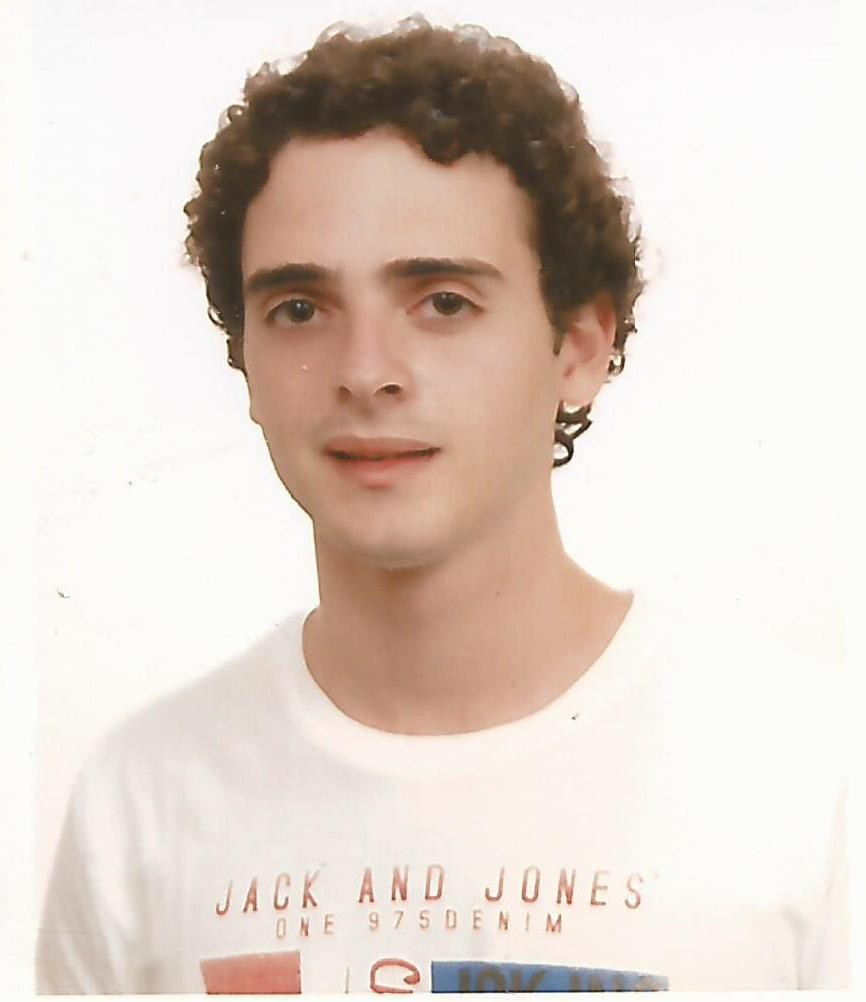
\includegraphics[width=1in,height=1.25in,clip,keepaspectratio]{foto_passe.jpg}}]{Gonçalo Fialho}
Vive em Rio de Mouro (Sintra). Estudou na Escola Secundária Leal da Câmara no Curso de Ciências e Tecnologias. Nos últimos 5 anos estudou no Instituto Superior Técnico e frequenta o Mestrado de Engenharia Infromática e de Computadores no campus da Alameda. 

Nos seus tempos livres gosta de sair com os amigos e jogar computador. 

Nos últimos 2 anos de faculdade fez parte da Junitec, Júnior Empresa do IST onde desempenhou funções no departamento técnico da empresa. 

Tem também um curso de Animação e durante as férias trabalha como Animador e Monitor de Colónias de Férias organizados pela Praznik.
\end{IEEEbiography}

\begin{IEEEbiography}[{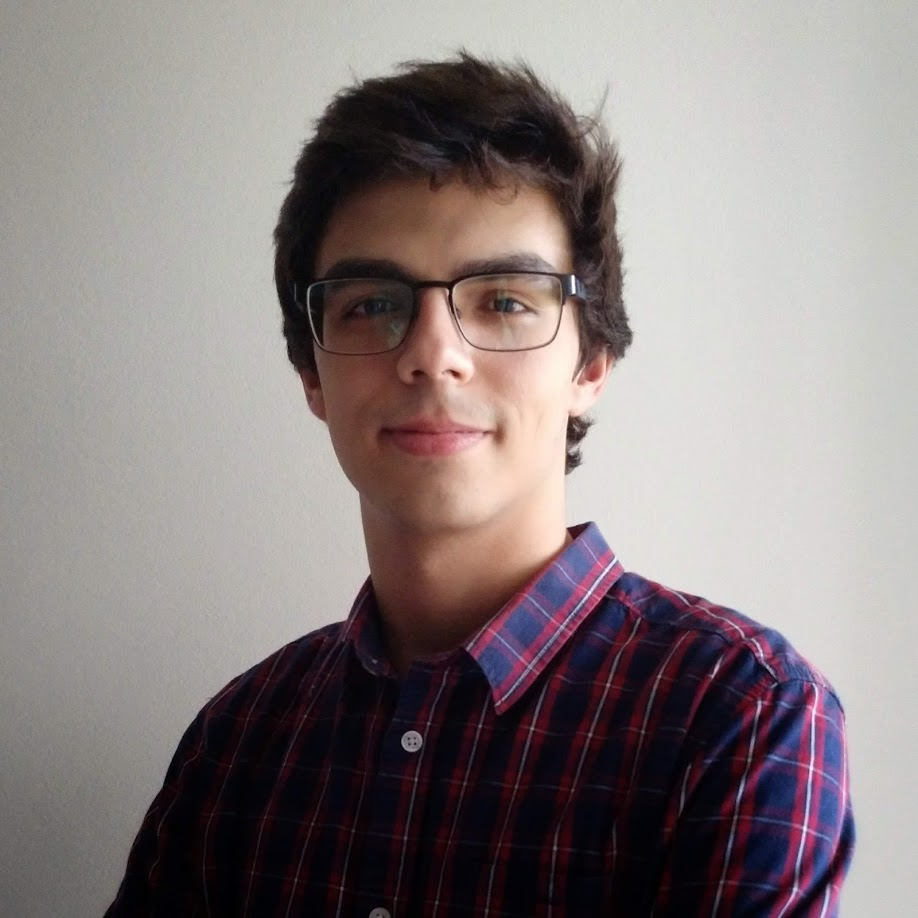
\includegraphics[width=1in,height=1.25in,clip,keepaspectratio]{foto_pedro.jpeg}}]{Pedro Duarte}
Estou de momento a acabar o Mestrado em Engenharia Informática e de Computadores no \textit{campus} da Alameda do Instituto Superior Técnico, com especialização em Sistemas Inteligentes e Sistemas da Informação. Tenho como \textit{hobby} a fotografia e os jogos de vídeo .O meu objetivo de vida é tornar o mundo um melhor lugar para todos os que vivem e irão viver nele. 
\end{IEEEbiography}



%%%%%%%%%%%%%%%%%%%%%%%%%%%%%%%%%%%%%%%%%%%%%%%%%%%%%%%%%%%%%%%%%%%%%%%%%%%%%%%%

%%%%%%%%%%%%%%%%%%%%%%%%%%%%%%%%%%%%%%%%%%%%%%%%%%%%%%%%%%%%%%%%%%%%%%%%%%%%%%%%
% APPENDIX WITH STATEMENT OF EXECUTION IS ONLY
% MANDATORY FOR SELF_INITIATIVE ACTIVITIES

%%%%%%%%%%%%%%%%%%%%%%%%%%%%%%%%%%%%%%%%%%%%%%%%%%%%%%%%%%%%%%%%%%%%%%%%%%%%%%%%
% *** DEFINITION OF ACRONYMS ***
	\acrodef{CPU}{Central Processing Unit}
	\acrodef{GUI}{Graphical User Interface}
	\acrodef{HTTP}{Hypertext Transfer Protocol}
	\acrodef{IST}{Instituto Superior Técnico}	
	\acrodef{LAN}{Local Area Network}
	\acrodef{PC}{Personal Computer}
	\acrodef{URL}{Uniform Resource Locator}
	\acrodef{VoD}{Video-on-demand}
	\acrodefplural{VoD}[VoDs]{Videos-on-demand}
	\acrodef{VoIP}{Voice over IP}
	\acrodef{WAN}{Wide Area Network}
	\acrodef{WLAN}{Wireless Local Area Network}
	\acrodef{WWAN}{Wireless Wide Area Network}
	\acrodef{WWW}{World Wide Web}
	
% that's all folks
\end{document}